\documentclass{article}
\usepackage[margin=1in, top = .8in, left=.8in]{geometry}
\usepackage{comment}
\usepackage{amsmath, amssymb}
\usepackage{framed}
\usepackage{enumerate}
\usepackage{comment}
\usepackage{tikz,pgfplots}
\usepgfplotslibrary{fillbetween}
\pgfplotsset{compat=1.15}
\usepackage[hyphens]{url}

\begin{document}

\begin{center}
    \large \textbf{Homework 6}
\end{center}
    %\item[\textbf{Week 6}]
                \begin{enumerate}
                    \item Consider the function
                    $$G(x) = \int_0^x 4-t^2+5t\,dt$$
                    \begin{enumerate}
                        \item On what intervals is $G(x)$ increasing?
                        \item At what value of $x$ is $G(x)$ increasing the fastest?
                        \item At what values of $x$ is $G(x)=0$?
                        \item What is the absolute maximum value of $G(x)$ on the interval $x \in [0,\infty)$? Give complete reasoning.
                    \end{enumerate}
                    \item Compute
                    $$\frac{d}{dx} \int_{\ln{x}}^{e^{x^2}} \frac{t^3}{t^2+1}\,dt$$
                    \item Let $p(x)$ be a constant $c$ on the interval $[0,2]$, and $0$ elsewhere.
                    \begin{enumerate}
                        \item If $p(x)$ is a probability density function, then what is the value of the constant $c$?
                        \item Find a formula for the cumulative distribution function $\displaystyle P(x)=\int_0^x p(t)\,dt$. Write the answer as a piecewise function. 
                        \item Graph $P(x)$.
                        
                    \end{enumerate}
                \item The following is a graph of a function $g(x)$, which is a probability density function. The function $g(x)$ is $0$ on $(-\infty,0]$ and $[4,\infty)$.
                        \begin{center}
        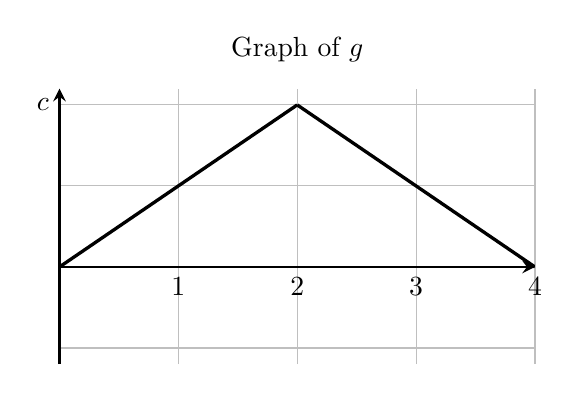
\begin{tikzpicture}
        \begin{axis}[
   	        xmin=0, xmax=4,
	        ymin=-1.2, ymax=2.2,
	        major tick length={0},
	        line width=1pt,
	        %xticks = {0,1,2,3,4},
 	        axis lines=center, height=2 in, width=3 in, grid=major,
 	        title = Graph of $g$,
 	        yticklabels = {, , ,,$c$}
	        ]
	    \addplot [black, smooth, very thick] plot coordinates {(0,0)(2,2)};
	    \addplot [black, smooth, very thick] plot coordinates {(2,2)(4,0)};

        \end{axis}
        \end{tikzpicture}
        \end{center}
                \begin{enumerate}
                    \item Find the value of $c$ needed to make $g$ a probability density function. thus determining the scale on the $y$-axis of the graph.
                    \item Write the formula for the cumulative distribution function as a piecewise function.
                    \item Graph the cumulative distribution function.
                    \item Find the probability that a number with this distribution lies between $3$ and $4$.
                \end{enumerate} 
                    \item Evaluate the following limits.
                        \begin{enumerate}
                            \item $\displaystyle \lim_{x\rightarrow \infty} \frac{\ln(\frac{1}{x})}{e^x}$
                            \item $\displaystyle \lim_{x\rightarrow \infty} \frac{\sqrt{x^2+6x}}{x}$
                            \item $\displaystyle\lim_{x \rightarrow 0} \frac{1}{x\ln{x}}$
                            \item $\displaystyle \lim_{x \rightarrow 1} \left(\frac{x}{x-1} - \frac{1}{\ln{x}}\right)$
                        \end{enumerate}
                    \item Two of the following integrals can be evaluated in closed form. Determine which two and evaluate them. 
                        \begin{itemize}
                            \item $\displaystyle \int_0^\infty e^{-x^2}\,dx$
                            \item $\displaystyle \int_0^\infty xe^{-x^2}\,dx$
                            \item $\displaystyle \int_0^\infty x^2e^{-x^2}\,dx$
                            \item $\displaystyle \int_0^\infty x^3e^{-x^2}\,dx$
                        \end{itemize}
                    \item Evaluate the integral.  If it is convergent, then determine its value.  Otherwise, show that it is divergent.
                        \begin{enumerate}
                            \item $\displaystyle \int_9^\infty \frac{5x}{x^2\sqrt{x}}\,dx$
                            \item $\displaystyle \int_9^\infty \frac{5x}{x\sqrt{x}}\,dx$
                            \item $\displaystyle \int_1^\infty e^{-7x}\, dx$
                            \item $\displaystyle \int_{0}^1 \frac{x^2}{x^3-1}\, dx$
                            \item $\displaystyle \int_{0}^2 \frac {3}{(x-1)^{2/3}}\, dx$
                            \item $\displaystyle \int_0^\infty \frac{1}{x\ln{x}}\,dx$
                        \end{enumerate}
                \end{enumerate}
                
\end{document}